%===========================================================
% This is the thesis template for the Statistics major at
% Amherst College. Brittney E. Bailey (bebailey@amherst.edu)
% adapted this template from the Reed College LaTeX thesis
% template in January 2019 with major updates in April 2020.
% Please send any comments/suggestions: bebailey@amherst.edu

% Most of the work for the original document class was done
% by Sam Noble (SN), as well as this template. Later comments
% etc. by Ben Salzberg (BTS). Additional restructuring and
% APA support by Jess Youngberg (JY). Email: cus@reed.edu
%===========================================================

\documentclass[12pt, twoside]{amherstthesis}
\usepackage{graphicx,latexsym}
\usepackage{amsmath}
\usepackage{amssymb,amsthm}
\usepackage{longtable,booktabs} %setspace loaded in .cls
\usepackage[hyphens]{url}
\usepackage{hyperref}
\usepackage{lmodern}
\usepackage{float}
\floatplacement{figure}{H}
\usepackage{rotating}
\usepackage{fancyvrb}
% User-added packages:
% End user-added packages

%===========================================================
% BIBLIOGRAPHY FORMATTING

% Next line commented out by CII
%%% \usepackage{natbib}
% Comment out the natbib line above and uncomment the
% following two lines to use the new biblatex-chicago style,
% for Chicago A. Also make some changes at the end where the
% bibliography is included.
%\usepackage{biblatex-chicago}
%\bibliography{thesis}


%===========================================================
% HYPERLINK FORMATTING

% Added by CII (Thanks, Hadley!)
% Use ref for internal links
\renewcommand{\hyperref}[2][???]{\autoref{#1}}
\def\chapterautorefname{Chapter}
\def\sectionautorefname{Section}
\def\subsectionautorefname{Subsection}
% End of CII addition
\usepackage{xcolor}
\hypersetup{
    colorlinks,
    linkcolor={red!50!black},
    citecolor={blue!50!black},
    urlcolor={blue!80!black}
}

%===========================================================
% CAPTION FORMATTING

% Added by CII
\usepackage{caption}
\captionsetup{width=5in}
% End of CII addition

%===========================================================
% TITLE FORMATTING

\renewcommand{\contentsname}{Table of Contents}

\usepackage{titlesec}
%%%%%%%%
% How to use titlesec:
% \titleformat{⟨command⟩}[⟨shape⟩]{⟨format⟩}{⟨label⟩}{⟨sep⟩}
%  {⟨before-code⟩}[⟨after-code⟩]
%%%%%%%%

\titleformat{\chapter}[hang]
{\normalfont%
    \Large% %change this size to your needs for the first line
    \bfseries}{\chaptertitlename\ \thechapter}{1em}{%
      %change this size to your needs for the second line
    }[]

\titleformat{\section}[hang]
{\normalfont%
    \large % %change this size to your needs for the first line
    \bfseries}{\thesection}{1em}{%
     %change this size to your needs for the second line
    }[]

\titleformat{\subsection}[hang]
{\normalfont%
    \normalsize % %change this size to your needs for the first line
    \bfseries}{\thesubsection}{1em}{%
     %change this size to your needs for the second line
    }[]

% \titleformat{\section}[display]
% {\normalfont%
%     \large% %change this size to your needs for the first line
%     \bfseries}{\chaptertitlename\ \thechapter}{20pt}{%
%     \normalsize %change this size to your needs for the second line
%     }


%===========================================================
% DOCUMENT FONT

% \usepackage{times}
% other fonts available eg: times, bookman, charter, palatino


%===========================================================
% PASSING FORMATS FROM RMD --> LATEX

%%%%%%%%
% NOTE: Dollar signs pass parameters between YAML inputs
% in index.Rmd and LaTeX
%%%%%%%%

\Abstract{
The abstract should be a short summary of your thesis work. A paragraph is usually sufficient here.
}

\Acknowledgments{
Use this space to thank those who have helped you in the thesis process (professors, staff, friends, family, etc.). If you had special funding to conduct your thesis work, that should be acknowledged here as well.
}

\Dedication{

}

\Preface{

}

% Formatting R code display
% Syntax highlighting #22

% Formatting R code: set baselinestretch = 1.5 for double-spacing
\DefineVerbatimEnvironment{Highlighting}{Verbatim}{
  baselinestretch = 1,
  commandchars=\\\{\}}

% Formatting R output display: set baselinestretch = 1.5 for double-spacing
\DefineVerbatimEnvironment{verbatim}{Verbatim}{
  baselinestretch = 1,
  % indent from left margin
  xleftmargin = 1mm,
  % vertical grey bar on left side of R output
  frame = leftline,
  framesep = 0pt,
  framerule = 1.5mm, rulecolor = \color{black!15}
  }

\title{My amazing title}
\author{Tony Ni}
\date{April DD, 20YY}
\division{}
\advisor{Brittney Bailey}
% for second advisor
\institution{Amherst College}
\degree{Bachelor of Arts}
\department{Mathematics and Statistics}

% Fix from pandoc about cslreferences?
% https://github.com/mpark/wg21/issues/54
\newlength{\cslhangindent}
\setlength{\cslhangindent}{1.5em}
\newenvironment{cslreferences}%
  {\setlength{\parindent}{0pt}%
  \everypar{\setlength{\hangindent}{\cslhangindent}}\ignorespaces}%
  {\par}

% Added by CII
%%% Copied from knitr
%% maxwidth is the original width if it's less than linewidth
%% otherwise use linewidth (to make sure the graphics do not exceed the margin)
\makeatletter
\def\maxwidth{ %
  \ifdim\Gin@nat@width>\linewidth
    \linewidth
  \else
    \Gin@nat@width
  \fi
}
\makeatother

% ===========================================
% DOCUMENT SPACING

\setlength{\parskip}{0pt}
% Added by CII

\providecommand{\tightlist}{%
  \setlength{\itemsep}{0pt}\setlength{\parskip}{0pt}}


% ===========================================
% ===========================================
% ===========================================
\begin{document}

\doublespace
% Everything below added by CII
  \maketitle

\frontmatter % this stuff will be roman-numbered
\pagenumbering{roman}
\pagestyle{fancyplain}
%\pagestyle{fancy} % this removes page numbers from the frontmatter

  \begin{abstract}
    The abstract should be a short summary of your thesis work. A paragraph is usually sufficient here.
  \end{abstract}
  \begin{acknowledgments}
    Use this space to thank those who have helped you in the thesis process (professors, staff, friends, family, etc.). If you had special funding to conduct your thesis work, that should be acknowledged here as well.
  \end{acknowledgments}

  \hypersetup{linkcolor=black}
  \setcounter{tocdepth}{2}
  \tableofcontents

  \addcontentsline{toc}{chapter}{List of Tables}\listoftables

  \addcontentsline{toc}{chapter}{List of Figures}\listoffigures


\mainmatter % here the regular arabic numbering starts
\pagenumbering{arabic}
\pagestyle{fancyplain} % turns page numbering back on

\hypertarget{intro}{%
\chapter{Introduction}\label{intro}}

The introduction should provide an overview of the work you set out to do and provide structure for the remainder of the document.

\hypertarget{background}{%
\section{Background}\label{background}}
\begin{itemize}
\item
  (coal ash report - car) coal one of the most dangerous combustible fossil fuels is comprised of a long list of dangerous chemicals -- including substances such as arsenic, radium, other carcinogens, metals that can impair developing children's brains, toxins dangerous to aquatic life, etc (Kelderman et al., 2019)
\item
  power plants produce 100mil tons of coal ash every year, which is dumped into landfills and waste ponds (Kelderman et al., 2019)
\item
  only recently (2015) have complaints and lawsuit arisen in which certain ecological organizations have attempted to sue the EPA to regulate disposal of coal ash (Kelderman et al., 2019)
\item
  this coal ash rule has forced power companies to make publicly available data regarding chemical concentrations in 265 coal plants containing ponds and landfills (about 3/4 of all coal power plants across the US) (Kelderman et al., 2019)
\item
  environmental agencies have concluded that the groundwater under basically all coal plants are contaminated (Kelderman et al., 2019)
\item
  HOWEVER this might be overstated? we wanted to investigate whether or not if this was true.
\end{itemize}
\begin{figure}

{\centering 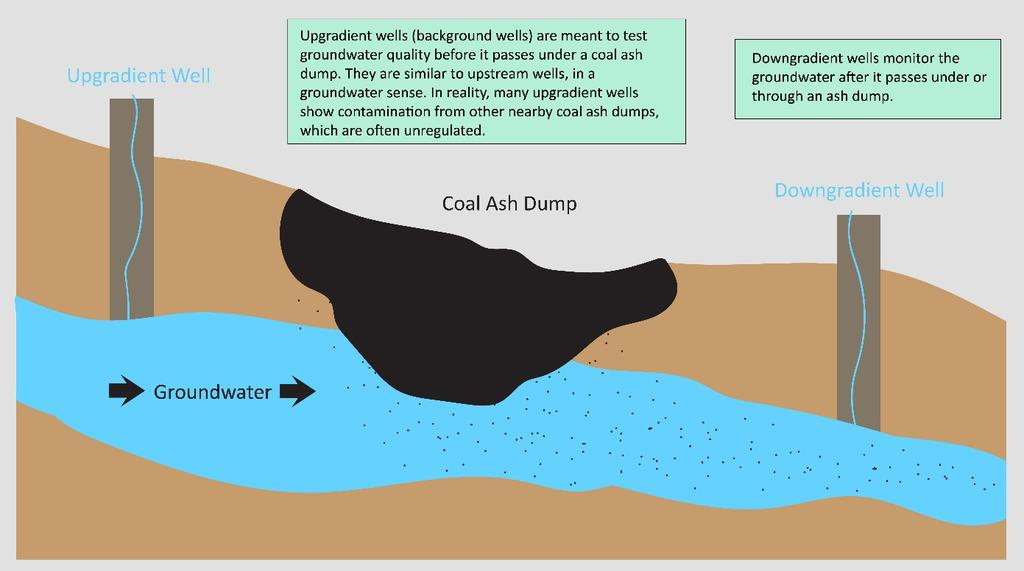
\includegraphics[width=1\linewidth]{figures/upgradientdowngradient} 

}

\caption{Difference Between Upgradient and Downgradient Wells}\label{fig:upgradientdowngradient}
\end{figure}
\begin{itemize}
\item
  upgradient wells (background wells) measures groundwater chemical levels BEFORE passing through a coal ash dump while downgradient wells monitor the groundwater AFTER it passes through an ash dump
\item
  we have reason to believe that many chemicals are NATURALLY OCCURING and as such, the statement made my environmental agencies regarding all groundwater being contaminated may be overstated
\item
  typically, we would estimate the amount of chemical contamination, for this example -- arsenic -- caused by a coal ash dump with the equation: downgradient arsenic concentration minus upgradient arsenic concentration
\item
  however, because there may be retired/unregulated upgradient wells that are occasionally contaminated already, this might be inaccurate
\end{itemize}
\begin{itemize}
\item
  END GOAL IS TO CORRECT THE CONTAMINATED VALUES
\item
  we have already conducted a preliminary investigation using a variety of machine learning techniques to aid us in identifying potential contaminated upgradient wells
\item
  we have also utilized bootstrapping and imputation techniques to correct for their measurements through by accounting for the innate contamination which may be caused by factors such as retired and unregulated wells
\item
  our methodologies have yet to account for another problem however, involving limit of detection problem which arises from the measuring devices' inability to obtain chemical concentrations smaller than a certain threshold amount
\end{itemize}
\hypertarget{data}{%
\section{Data}\label{data}}

\hypertarget{coalashrule}{%
\subsection{Coal Ash Rule}\label{coalashrule}}
\begin{itemize}
\item
  A large coal ash spill at the Tennessee Valley Authority (TVA) which occured on December 22, 2008 in Kingston, TN -- prompted the Environmental Protection Agency (EPA) to propose a set of standardized regulations and procedures to address the concerns regarding coal ash plants nationwide in the US (Environmental Protection Agency, 2020)
\item
  This was known as the Coal Ash Rule, passed on December 19, 2014 (Environmental Protection Agency, 2020)
\item
  Changes were made to the Coal Ash Rule over the years in the form of `amendments,' one of which made required facility information and data to be made publicaly available to the public (April 15, 2015 rule change) (Environmental Protection Agency, 2020)
\end{itemize}
\hypertarget{source-of-data}{%
\subsection{Source of Data}\label{source-of-data}}
\begin{itemize}
\item
  the data used in the study are from the results published in ``Annual Groundwater Monitoring and Corrective Action Reports'' which were made available to the public in March 2018 (Environmental Integrity Project, 2020)
\item
  these reports are in PDF format and are thousands of pages long, which makes it difficult for individuals to look through the data in a meaningful way (Environmental Integrity Project, 2020)
\item
  the EIP wranged the data into a more accessible machine-readable format which contains information from over 443 annual groundwater monitoring reports posted by 265 coal ash plants (Environmental Integrity Project, 2020)
\item
  they obtained the data from an online, publicly available database containing groundwater monitoring results from the first ``Annual Groundwater Monitoring and Corrective Action Reports'' in 2018 which was collected from coal plants and coal ash dumps under the Coal Ash Rule (Environmental Integrity Project, 2020)
\end{itemize}
\hypertarget{variables}{%
\subsection{Variables}\label{variables}}
\begin{itemize}
\item
  a coal ash site consists of multiple disposal areas
\item
  within these disposal areas lie multiple wells
\item
  each observation represents a well
\item
  wells are split into 2 different types - upgradient and downgradient wells
\item
  variables consist of information regard chemical contaminant concentrations and specifics regarding the well
\item
  from the 19 different contaminants (antimony, arsenic, boron, etc. \ldots) a major problem is that some wells only have measurements for certain chemicals and don't have them for others
\item
  we are currently using information from plants within illinois but there is data for all the states in the US
\end{itemize}
\hypertarget{methodology}{%
\chapter{Methodology}\label{methodology}}

\hypertarget{planofaction}{%
\section{Plan of Action}\label{planofaction}}
\begin{itemize}
\item
  we wanted to identify these contaminated upgradient wells and then ``correct'' these measurements
\item
  we will use manual code to flag contaminated vs noncontaminated wells (filter) using threshold values (this table is from coal ash pdf, but could make manual one)
\end{itemize}
\textbackslash begin\{figure\}

\{\centering 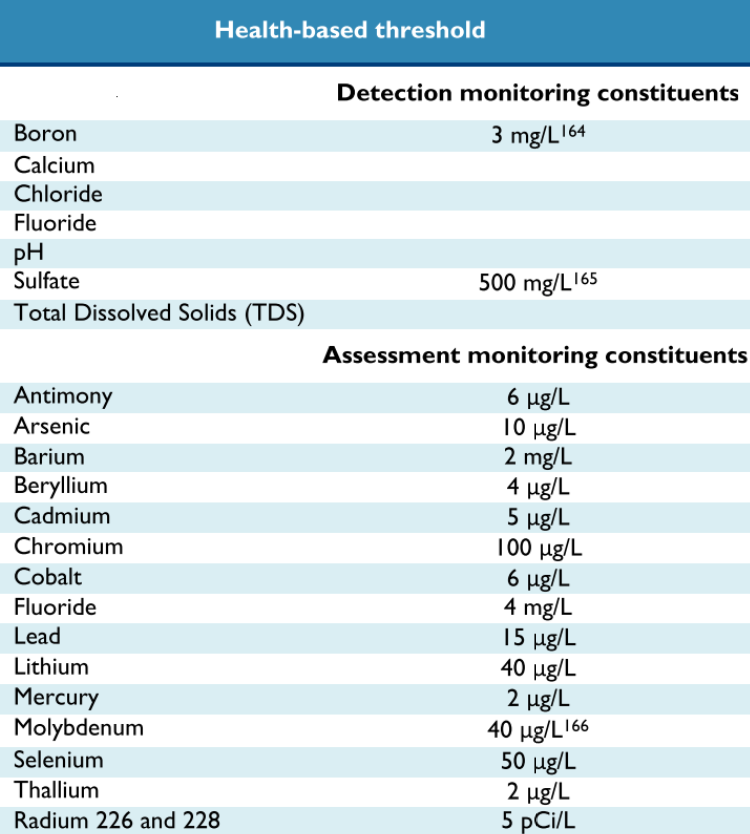
\includegraphics[width=1\linewidth]{figures/abridged_table1}

\}

\caption{Table of Threshold Values}

(\#fig:abridged\_table1)
\textbackslash end\{figure\}
\begin{itemize}
\item
  firstly, we used agglomerative hierarchical clustering to identify contaminated upgradient wells in our `illinois' dataset (thoughts, maybe we want to expand/use a bigger dataset) using Ward's Method
\item
  then, we separated our data into two parts -- one dataset containing these contaminated upgradient wells and another dataset containing UNcontaminated upgradient wells
\item
  then, we randomly sampled (with replacement) (500) times from the measurements of the chemical from non-contaminated upgradient wells to create an empirical distribution of naturally occurring chemical levels. this serves as the set of imputed ``corrected'' measurements of the chemical for each contaminated upgradient well
\item
  then, we identify the specific `disposal\_area' that the contaminated wells belong to and FILTERED to have a dataset contain only the downgradient wells that corresponded to the upgradient wells -- calculating the average of the downgradient wells (for the illinois dataset, we only had contaminated upgradient wells from TWO disposal areas)
\item
  finally, we subtracted each of the (500) imputed upgradient measurements from the average downgradient measure. This creates a distribution of (500) values of the contaminant concentrations caused by the disposal area.
\item
  we can then take the median of these (500) values as the estimate of the contamination caused by the disposal area (for the given chemical) and then use the 2.5 percentile and 97.5 percentile of the distribution as a bootstrap-type confidence interval.
\item
  we found that the first disposal area didn't have any obvious contamination b/c the difference that we calculated (upgrad - downgradient) was mostly 0, while for the second disposal area the different was much greater than 0
\end{itemize}
\hypertarget{clustering}{%
\section{Clustering}\label{clustering}}
\begin{itemize}
\item
  unsupervised ml task whose goal is to divide the data in to clusters without knowing what the groups will look like beforehand (Lantz, 2013)
\item
  used mainly for knowledge discovery rather than prediction (Lantz, 2013)
\item
  many different ways to go about conducting a clustering based investigation, k-means clustering is the method used to try to find relationships between the wells
\item
  our reasons to using this is to see whether if we can identify contaminated wells from uncontaminated wells (we don't anticipate it working due to the messed-up data, but MAYBE we would want to do some sort of study where we 1. run clustering with the messed up data and compare it to 2. run clustering with the corrected data (whatever that might be))
\end{itemize}
\hypertarget{kmeans}{%
\subsection{K-Means Clustering}\label{kmeans}}
\begin{itemize}
\item
  very popular and widely used clustering algorithm even since its inception decades ago (Lantz, 2013)
\item
  STRENGTHS: uses simple ideas to identify clsuters that can be explained in non-statistical terms, is flexible and has lots of parameters which can be adjusted to address its issues, and it is efficient (Lantz, 2013)
\item
  WEAKNESSES: not as sophisticated than some recent clustering techniques which have arisen recently, since it uses randomness within it, the clusters which it finds is not guaranteed to be optimal, requires a guess as to how many clusters may naturally exist in the data in order for the algorithm to run (Lantz, 2013)
\item
  HOW IT WORKS: (add in later, if relevant?)
\end{itemize}
\hypertarget{corrections}{%
\chapter*{Corrections}\label{corrections}}
\addcontentsline{toc}{chapter}{Corrections}

A list of corrections after submission to department.

Corrections may be made to the body of the thesis, but every such correction will be acknowledged in a list under the heading ``Corrections,'' along with the statement ``When originally submitted, this honors thesis contained some errors which have been corrected in the current version. Here is a list of the errors that were corrected.'' This list will be given on a sheet or sheets to be appended to the thesis. Corrections to spelling, grammar, or typography may be acknowledged by a general statement such as ``30 spellings were corrected in various places in the thesis, and the notation for definite integral was changed in approximately 10 places.'' However, any correction that affects the meaning of a sentence or paragraph should be described in careful detail. The files samplethesis.tex and samplethesis.pdf show what the ``Corrections'' section should look like. Questions about what should appear in the ``Corrections'' should be directed to the Chair.

\backmatter

\hypertarget{references}{%
\chapter*{References}\label{references}}
\addcontentsline{toc}{chapter}{References}

\noindent

\setlength{\parindent}{-0.20in}
\setlength{\leftskip}{0.20in}
\setlength{\parskip}{8pt}

\hypertarget{refs}{}
\begin{cslreferences}
\leavevmode\hypertarget{ref-EIP2020}{}%
Environmental Integrity Project. (2020). Coal Ash Groundwater Contamination: Documenting Coal Ash Pollution. Retrieved from \url{https://environmentalintegrity.org/coal-ash-groundwater-contamination/}

\leavevmode\hypertarget{ref-Car2020}{}%
Environmental Protection Agency. (2020). Disposal of Coal Combustion Residuals from Electric Utilities Rulemakings. Retrieved from \url{https://www.epa.gov/coalash/coal-ash-rule}

\leavevmode\hypertarget{ref-Kelderman2019}{}%
Kelderman, K., Kunstman, B., Roy, H., Sivakumar, N., Mccormick, S., \& Bernhardt, C. (2019). Coal's Poisonous Legacy: Groundwater Contaminated by Coal Ash Across the U.S.

\leavevmode\hypertarget{ref-Lantz2013}{}%
Lantz, B. (2013). \emph{Machine Learning with R}. Birmingham: Packt Publishing.
\end{cslreferences}
% Index?

\end{document}
